\documentclass[twoside]{book}

% Packages required by doxygen
\usepackage{fixltx2e}
\usepackage{calc}
\usepackage{doxygen}
\usepackage[export]{adjustbox} % also loads graphicx
\usepackage{graphicx}
\usepackage[utf8]{inputenc}
\usepackage{makeidx}
\usepackage{multicol}
\usepackage{multirow}
\PassOptionsToPackage{warn}{textcomp}
\usepackage{textcomp}
\usepackage[nointegrals]{wasysym}
\usepackage[table]{xcolor}

% Font selection
\usepackage[T1]{fontenc}
\usepackage[scaled=.90]{helvet}
\usepackage{courier}
\usepackage{amssymb}
\usepackage{sectsty}
\renewcommand{\familydefault}{\sfdefault}
\allsectionsfont{%
  \fontseries{bc}\selectfont%
  \color{darkgray}%
}
\renewcommand{\DoxyLabelFont}{%
  \fontseries{bc}\selectfont%
  \color{darkgray}%
}
\newcommand{\+}{\discretionary{\mbox{\scriptsize$\hookleftarrow$}}{}{}}

% Page & text layout
\usepackage{geometry}
\geometry{%
  a4paper,%
  top=2.5cm,%
  bottom=2.5cm,%
  left=2.5cm,%
  right=2.5cm%
}
\tolerance=750
\hfuzz=15pt
\hbadness=750
\setlength{\emergencystretch}{15pt}
\setlength{\parindent}{0cm}
\setlength{\parskip}{3ex plus 2ex minus 2ex}
\makeatletter
\renewcommand{\paragraph}{%
  \@startsection{paragraph}{4}{0ex}{-1.0ex}{1.0ex}{%
    \normalfont\normalsize\bfseries\SS@parafont%
  }%
}
\renewcommand{\subparagraph}{%
  \@startsection{subparagraph}{5}{0ex}{-1.0ex}{1.0ex}{%
    \normalfont\normalsize\bfseries\SS@subparafont%
  }%
}
\makeatother

% Headers & footers
\usepackage{fancyhdr}
\pagestyle{fancyplain}
\fancyhead[LE]{\fancyplain{}{\bfseries\thepage}}
\fancyhead[CE]{\fancyplain{}{}}
\fancyhead[RE]{\fancyplain{}{\bfseries\leftmark}}
\fancyhead[LO]{\fancyplain{}{\bfseries\rightmark}}
\fancyhead[CO]{\fancyplain{}{}}
\fancyhead[RO]{\fancyplain{}{\bfseries\thepage}}
\fancyfoot[LE]{\fancyplain{}{}}
\fancyfoot[CE]{\fancyplain{}{}}
\fancyfoot[RE]{\fancyplain{}{\bfseries\scriptsize Generated by Doxygen }}
\fancyfoot[LO]{\fancyplain{}{\bfseries\scriptsize Generated by Doxygen }}
\fancyfoot[CO]{\fancyplain{}{}}
\fancyfoot[RO]{\fancyplain{}{}}
\renewcommand{\footrulewidth}{0.4pt}
\renewcommand{\chaptermark}[1]{%
  \markboth{#1}{}%
}
\renewcommand{\sectionmark}[1]{%
  \markright{\thesection\ #1}%
}

% Indices & bibliography
\usepackage{natbib}
\usepackage[titles]{tocloft}
\setcounter{tocdepth}{3}
\setcounter{secnumdepth}{5}
\makeindex

% Hyperlinks (required, but should be loaded last)
\usepackage{ifpdf}
\ifpdf
  \usepackage[pdftex,pagebackref=true]{hyperref}
\else
  \usepackage[ps2pdf,pagebackref=true]{hyperref}
\fi
\hypersetup{%
  colorlinks=true,%
  linkcolor=blue,%
  citecolor=blue,%
  unicode%
}

% Custom commands
\newcommand{\clearemptydoublepage}{%
  \newpage{\pagestyle{empty}\cleardoublepage}%
}

\usepackage{caption}
\captionsetup{labelsep=space,justification=centering,font={bf},singlelinecheck=off,skip=4pt,position=top}

%===== C O N T E N T S =====

\begin{document}

% Titlepage & ToC
\hypersetup{pageanchor=false,
             bookmarksnumbered=true,
             pdfencoding=unicode
            }
\pagenumbering{roman}
\begin{titlepage}
\vspace*{7cm}
\begin{center}%
{\Large Background\+Subtractor\+C\+NT \\[1ex]\large 1.\+1.\+1 }\\
\vspace*{1cm}
{\large Generated by Doxygen 1.8.11}\\
\end{center}
\end{titlepage}
\clearemptydoublepage
\tableofcontents
\clearemptydoublepage
\pagenumbering{arabic}
\hypersetup{pageanchor=true}

%--- Begin generated contents ---
\chapter{Usage in a nutshell}
\label{index}\hypertarget{index}{}This is a drop in replacement A\+PI for the background subtraction solutions supplied with Open\+CV 3.\+1.\+0 and above. See these drop in replacement examples for C++ in \hyperlink{main_8cpp-example}{main.cpp} file, and for python in \hyperlink{python_2demo_8py-example}{demo.py} file.

\subsubsection*{Usage tuning}

This module is very predictable as it\textquotesingle{}s behavior follows common sense. You can tune the behavior when the Background\+Subtractor is created (or later with setters) –


\begin{DoxyCode}
1 Ptr<BackgroundSubtractorCNT>
2 createBackgroundSubtractorCNT(int minPixelStability = 15,
3                               bool useHistory = true,
4                               int maxPixelStability = 15*60,
5                               bool isParallel = true);
\end{DoxyCode}

\begin{DoxyItemize}
\item Use your estimated F\+PS as the base for tuning, as explained below (it doesn’t have to be accurate).
\item Each of these parameters can be evaluated according to these guidelines\+:
\end{DoxyItemize}

\paragraph*{How long to wait before considering a pixel to be a background?}

When you and I look at a scene, we wait for some time before we consider an item to be part of a background. The assumption here is that it takes about 1 second, but you can play with it. I recommend using your expected F\+PS as the value of min\+Pixel\+Stability when using \hyperlink{bgsubcnt_8h_a6a6efd913954320be33f39c32a4c5a7e}{create\+Background\+Subtractor\+C\+N\+T()}. The value represents the number of frames to wait when a pixel is not changing before marking it as background. The demo is doing exactly that in main.\+cpp.

\paragraph*{How long to wait before recognizing the background changed?}

Okay – so we’ve set something to be a background, and things are passing in front of it. When something is in front of it for a long time, then it’s time to treat it as a background instead of the previous one, but how long to wait before doing this replacement? The algorithm here was tested with a 60 seconds value and gave good results. You can change that as you want, but I recommend setting max\+Pixel\+Stability to “min\+Pixel\+Stability$\ast$60″ in \hyperlink{bgsubcnt_8h_a6a6efd913954320be33f39c32a4c5a7e}{create\+Background\+Subtractor\+C\+N\+T()}. The demo is doing exactly that in main.\+cpp.

\paragraph*{But what if you want to R\+E\+A\+CT V\+E\+RY F\+A\+ST TO S\+C\+E\+NE C\+H\+A\+N\+G\+ES?}

If reducing max\+Pixel\+Stability is not enough, you can use ‘false‘ for use\+History in \hyperlink{bgsubcnt_8h_a6a6efd913954320be33f39c32a4c5a7e}{create\+Background\+Subtractor\+C\+N\+T()}. In this case max\+Pixel\+Stability is ignored. Because the background distinction is weaker, you’ll see small ghosts following your foreground objects and the background image will have some ghosts images fading in it. Using “min\+Pixel\+Stability=F\+P\+S/5” will reduce this phenomena.

\paragraph*{To parallel or not to parallel?}

In my experience paralleling everything automatically is a double edged sword. On one hand you don’t need to worry about optimizations if you have enough processing power. On the other hand, splitting your processing carefully can yield a better optimization. I leave this to you to experiment and decide for your specific design. 
\chapter{Hierarchical Index}
\section{Class Hierarchy}
This inheritance list is sorted roughly, but not completely, alphabetically\+:\begin{DoxyCompactList}
\item Background\+Subtractor\begin{DoxyCompactList}
\item \contentsline{section}{cv\+:\+:bgsubcnt\+:\+:Background\+Subtractor\+C\+NT}{\pageref{classcv_1_1bgsubcnt_1_1BackgroundSubtractorCNT}}{}
\end{DoxyCompactList}
\end{DoxyCompactList}

\chapter{Class Index}
\section{Class List}
Here are the classes, structs, unions and interfaces with brief descriptions\+:\begin{DoxyCompactList}
\item\contentsline{section}{\hyperlink{classcv_1_1bgsubcnt_1_1BackgroundSubtractorCNT}{cv\+::bgsubcnt\+::\+Background\+Subtractor\+C\+NT} \\*Background subtraction based on counting. About as fast as M\+O\+G2 on a high end system. More than twice faster than M\+O\+G2 on cheap hardware (benchmarked on Raspberry Pi3). Algorithm by Sagi Zeevi }{\pageref{classcv_1_1bgsubcnt_1_1BackgroundSubtractorCNT}}{}
\end{DoxyCompactList}

\chapter{File Index}
\section{File List}
Here is a list of all documented files with brief descriptions\+:\begin{DoxyCompactList}
\item\contentsline{section}{Background\+Subtractor\+C\+N\+T/\hyperlink{bgsubcnt_8h}{bgsubcnt.\+h} }{\pageref{bgsubcnt_8h}}{}
\end{DoxyCompactList}

\chapter{Class Documentation}
\hypertarget{classcv_1_1bgsubcnt_1_1BackgroundSubtractorCNT}{}\section{cv\+:\+:bgsubcnt\+:\+:Background\+Subtractor\+C\+NT Class Reference}
\label{classcv_1_1bgsubcnt_1_1BackgroundSubtractorCNT}\index{cv\+::bgsubcnt\+::\+Background\+Subtractor\+C\+NT@{cv\+::bgsubcnt\+::\+Background\+Subtractor\+C\+NT}}


Background subtraction based on counting. About as fast as M\+O\+G2 on a high end system. More than twice faster than M\+O\+G2 on cheap hardware (benchmarked on Raspberry Pi3). Algorithm by Sagi Zeevi.  




{\ttfamily \#include $<$bgsubcnt.\+h$>$}

Inheritance diagram for cv\+:\+:bgsubcnt\+:\+:Background\+Subtractor\+C\+NT\+:\begin{figure}[H]
\begin{center}
\leavevmode
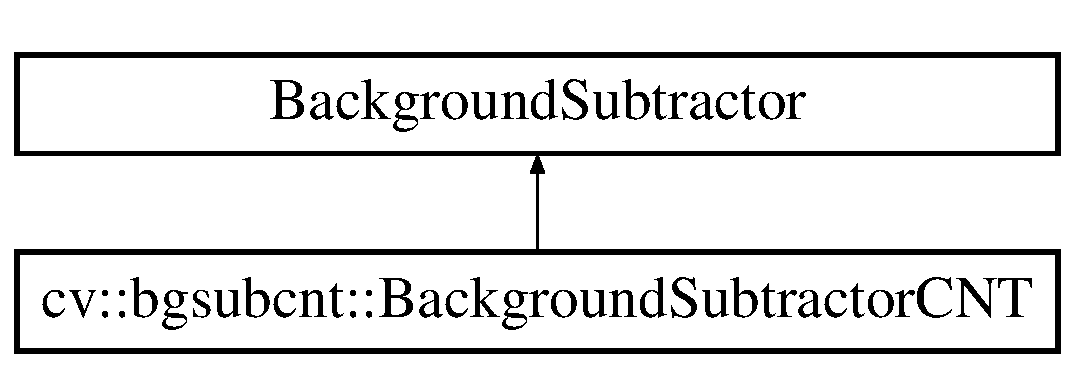
\includegraphics[height=2.000000cm]{classcv_1_1bgsubcnt_1_1BackgroundSubtractorCNT}
\end{center}
\end{figure}
\subsection*{Public Member Functions}
\begin{DoxyCompactItemize}
\item 
virtual C\+V\+\_\+\+W\+R\+AP int \hyperlink{classcv_1_1bgsubcnt_1_1BackgroundSubtractorCNT_ae989dd01f33c289a21b995ee9c69c600}{get\+Min\+Pixel\+Stability} () const =0
\item 
virtual C\+V\+\_\+\+W\+R\+AP void \hyperlink{classcv_1_1bgsubcnt_1_1BackgroundSubtractorCNT_a7fe9be675d4c1995123a60d56db75422}{set\+Min\+Pixel\+Stability} (int value)=0
\item 
virtual C\+V\+\_\+\+W\+R\+AP int \hyperlink{classcv_1_1bgsubcnt_1_1BackgroundSubtractorCNT_ac45a2faa6b753624cbbff9d341cdd3db}{get\+Max\+Pixel\+Stability} () const =0
\item 
virtual C\+V\+\_\+\+W\+R\+AP void \hyperlink{classcv_1_1bgsubcnt_1_1BackgroundSubtractorCNT_a3414551506bf27dda254dd245bfa8e03}{set\+Max\+Pixel\+Stability} (int value)=0
\begin{DoxyCompactList}\small\item\em see \end{DoxyCompactList}\item 
virtual C\+V\+\_\+\+W\+R\+AP bool \hyperlink{classcv_1_1bgsubcnt_1_1BackgroundSubtractorCNT_a86315a974023e507fdc7a40bba177399}{get\+Use\+History} () const =0
\item 
virtual C\+V\+\_\+\+W\+R\+AP void \hyperlink{classcv_1_1bgsubcnt_1_1BackgroundSubtractorCNT_ab2da57637e04beecbe8d812e00a54c52}{set\+Use\+History} (bool value)=0
\item 
virtual C\+V\+\_\+\+W\+R\+AP bool \hyperlink{classcv_1_1bgsubcnt_1_1BackgroundSubtractorCNT_a2e31e009b3901e4a1e43edf7e87cba51}{get\+Is\+Parallel} () const =0
\item 
virtual C\+V\+\_\+\+W\+R\+AP void \hyperlink{classcv_1_1bgsubcnt_1_1BackgroundSubtractorCNT_ab7d88f5d064b3c5cb0a18e80bd0bc265}{set\+Is\+Parallel} (bool value)=0
\end{DoxyCompactItemize}


\subsection{Detailed Description}
\begin{DoxySeeAlso}{See also}
\hyperlink{bgsubcnt_8h_a6a6efd913954320be33f39c32a4c5a7e}{create\+Background\+Subtractor\+C\+N\+T()} 
\end{DoxySeeAlso}


\subsection{Member Function Documentation}
\index{cv\+::bgsubcnt\+::\+Background\+Subtractor\+C\+NT@{cv\+::bgsubcnt\+::\+Background\+Subtractor\+C\+NT}!get\+Is\+Parallel@{get\+Is\+Parallel}}
\index{get\+Is\+Parallel@{get\+Is\+Parallel}!cv\+::bgsubcnt\+::\+Background\+Subtractor\+C\+NT@{cv\+::bgsubcnt\+::\+Background\+Subtractor\+C\+NT}}
\subsubsection[{\texorpdfstring{get\+Is\+Parallel() const =0}{getIsParallel() const =0}}]{\setlength{\rightskip}{0pt plus 5cm}virtual C\+V\+\_\+\+W\+R\+AP bool cv\+::bgsubcnt\+::\+Background\+Subtractor\+C\+N\+T\+::get\+Is\+Parallel (
\begin{DoxyParamCaption}
{}
\end{DoxyParamCaption}
) const\hspace{0.3cm}{\ttfamily [pure virtual]}}\hypertarget{classcv_1_1bgsubcnt_1_1BackgroundSubtractorCNT_a2e31e009b3901e4a1e43edf7e87cba51}{}\label{classcv_1_1bgsubcnt_1_1BackgroundSubtractorCNT_a2e31e009b3901e4a1e43edf7e87cba51}
\begin{DoxySeeAlso}{See also}
\hyperlink{bgsubcnt_8h_a6a6efd913954320be33f39c32a4c5a7e}{create\+Background\+Subtractor\+C\+N\+T()} 
\end{DoxySeeAlso}
\index{cv\+::bgsubcnt\+::\+Background\+Subtractor\+C\+NT@{cv\+::bgsubcnt\+::\+Background\+Subtractor\+C\+NT}!get\+Max\+Pixel\+Stability@{get\+Max\+Pixel\+Stability}}
\index{get\+Max\+Pixel\+Stability@{get\+Max\+Pixel\+Stability}!cv\+::bgsubcnt\+::\+Background\+Subtractor\+C\+NT@{cv\+::bgsubcnt\+::\+Background\+Subtractor\+C\+NT}}
\subsubsection[{\texorpdfstring{get\+Max\+Pixel\+Stability() const =0}{getMaxPixelStability() const =0}}]{\setlength{\rightskip}{0pt plus 5cm}virtual C\+V\+\_\+\+W\+R\+AP int cv\+::bgsubcnt\+::\+Background\+Subtractor\+C\+N\+T\+::get\+Max\+Pixel\+Stability (
\begin{DoxyParamCaption}
{}
\end{DoxyParamCaption}
) const\hspace{0.3cm}{\ttfamily [pure virtual]}}\hypertarget{classcv_1_1bgsubcnt_1_1BackgroundSubtractorCNT_ac45a2faa6b753624cbbff9d341cdd3db}{}\label{classcv_1_1bgsubcnt_1_1BackgroundSubtractorCNT_ac45a2faa6b753624cbbff9d341cdd3db}
\begin{DoxySeeAlso}{See also}
\hyperlink{bgsubcnt_8h_a6a6efd913954320be33f39c32a4c5a7e}{create\+Background\+Subtractor\+C\+N\+T()} 
\end{DoxySeeAlso}
\index{cv\+::bgsubcnt\+::\+Background\+Subtractor\+C\+NT@{cv\+::bgsubcnt\+::\+Background\+Subtractor\+C\+NT}!get\+Min\+Pixel\+Stability@{get\+Min\+Pixel\+Stability}}
\index{get\+Min\+Pixel\+Stability@{get\+Min\+Pixel\+Stability}!cv\+::bgsubcnt\+::\+Background\+Subtractor\+C\+NT@{cv\+::bgsubcnt\+::\+Background\+Subtractor\+C\+NT}}
\subsubsection[{\texorpdfstring{get\+Min\+Pixel\+Stability() const =0}{getMinPixelStability() const =0}}]{\setlength{\rightskip}{0pt plus 5cm}virtual C\+V\+\_\+\+W\+R\+AP int cv\+::bgsubcnt\+::\+Background\+Subtractor\+C\+N\+T\+::get\+Min\+Pixel\+Stability (
\begin{DoxyParamCaption}
{}
\end{DoxyParamCaption}
) const\hspace{0.3cm}{\ttfamily [pure virtual]}}\hypertarget{classcv_1_1bgsubcnt_1_1BackgroundSubtractorCNT_ae989dd01f33c289a21b995ee9c69c600}{}\label{classcv_1_1bgsubcnt_1_1BackgroundSubtractorCNT_ae989dd01f33c289a21b995ee9c69c600}
\begin{DoxySeeAlso}{See also}
\hyperlink{bgsubcnt_8h_a6a6efd913954320be33f39c32a4c5a7e}{create\+Background\+Subtractor\+C\+N\+T()} 
\end{DoxySeeAlso}
\index{cv\+::bgsubcnt\+::\+Background\+Subtractor\+C\+NT@{cv\+::bgsubcnt\+::\+Background\+Subtractor\+C\+NT}!get\+Use\+History@{get\+Use\+History}}
\index{get\+Use\+History@{get\+Use\+History}!cv\+::bgsubcnt\+::\+Background\+Subtractor\+C\+NT@{cv\+::bgsubcnt\+::\+Background\+Subtractor\+C\+NT}}
\subsubsection[{\texorpdfstring{get\+Use\+History() const =0}{getUseHistory() const =0}}]{\setlength{\rightskip}{0pt plus 5cm}virtual C\+V\+\_\+\+W\+R\+AP bool cv\+::bgsubcnt\+::\+Background\+Subtractor\+C\+N\+T\+::get\+Use\+History (
\begin{DoxyParamCaption}
{}
\end{DoxyParamCaption}
) const\hspace{0.3cm}{\ttfamily [pure virtual]}}\hypertarget{classcv_1_1bgsubcnt_1_1BackgroundSubtractorCNT_a86315a974023e507fdc7a40bba177399}{}\label{classcv_1_1bgsubcnt_1_1BackgroundSubtractorCNT_a86315a974023e507fdc7a40bba177399}
\begin{DoxySeeAlso}{See also}
\hyperlink{bgsubcnt_8h_a6a6efd913954320be33f39c32a4c5a7e}{create\+Background\+Subtractor\+C\+N\+T()} 
\end{DoxySeeAlso}
\index{cv\+::bgsubcnt\+::\+Background\+Subtractor\+C\+NT@{cv\+::bgsubcnt\+::\+Background\+Subtractor\+C\+NT}!set\+Is\+Parallel@{set\+Is\+Parallel}}
\index{set\+Is\+Parallel@{set\+Is\+Parallel}!cv\+::bgsubcnt\+::\+Background\+Subtractor\+C\+NT@{cv\+::bgsubcnt\+::\+Background\+Subtractor\+C\+NT}}
\subsubsection[{\texorpdfstring{set\+Is\+Parallel(bool value)=0}{setIsParallel(bool value)=0}}]{\setlength{\rightskip}{0pt plus 5cm}virtual C\+V\+\_\+\+W\+R\+AP void cv\+::bgsubcnt\+::\+Background\+Subtractor\+C\+N\+T\+::set\+Is\+Parallel (
\begin{DoxyParamCaption}
\item[{bool}]{value}
\end{DoxyParamCaption}
)\hspace{0.3cm}{\ttfamily [pure virtual]}}\hypertarget{classcv_1_1bgsubcnt_1_1BackgroundSubtractorCNT_ab7d88f5d064b3c5cb0a18e80bd0bc265}{}\label{classcv_1_1bgsubcnt_1_1BackgroundSubtractorCNT_ab7d88f5d064b3c5cb0a18e80bd0bc265}
\begin{DoxySeeAlso}{See also}
\hyperlink{bgsubcnt_8h_a6a6efd913954320be33f39c32a4c5a7e}{create\+Background\+Subtractor\+C\+N\+T()} 
\end{DoxySeeAlso}
\index{cv\+::bgsubcnt\+::\+Background\+Subtractor\+C\+NT@{cv\+::bgsubcnt\+::\+Background\+Subtractor\+C\+NT}!set\+Max\+Pixel\+Stability@{set\+Max\+Pixel\+Stability}}
\index{set\+Max\+Pixel\+Stability@{set\+Max\+Pixel\+Stability}!cv\+::bgsubcnt\+::\+Background\+Subtractor\+C\+NT@{cv\+::bgsubcnt\+::\+Background\+Subtractor\+C\+NT}}
\subsubsection[{\texorpdfstring{set\+Max\+Pixel\+Stability(int value)=0}{setMaxPixelStability(int value)=0}}]{\setlength{\rightskip}{0pt plus 5cm}virtual C\+V\+\_\+\+W\+R\+AP void cv\+::bgsubcnt\+::\+Background\+Subtractor\+C\+N\+T\+::set\+Max\+Pixel\+Stability (
\begin{DoxyParamCaption}
\item[{int}]{value}
\end{DoxyParamCaption}
)\hspace{0.3cm}{\ttfamily [pure virtual]}}\hypertarget{classcv_1_1bgsubcnt_1_1BackgroundSubtractorCNT_a3414551506bf27dda254dd245bfa8e03}{}\label{classcv_1_1bgsubcnt_1_1BackgroundSubtractorCNT_a3414551506bf27dda254dd245bfa8e03}
\begin{DoxySeeAlso}{See also}
\hyperlink{bgsubcnt_8h_a6a6efd913954320be33f39c32a4c5a7e}{create\+Background\+Subtractor\+C\+N\+T()} 
\end{DoxySeeAlso}
\index{cv\+::bgsubcnt\+::\+Background\+Subtractor\+C\+NT@{cv\+::bgsubcnt\+::\+Background\+Subtractor\+C\+NT}!set\+Min\+Pixel\+Stability@{set\+Min\+Pixel\+Stability}}
\index{set\+Min\+Pixel\+Stability@{set\+Min\+Pixel\+Stability}!cv\+::bgsubcnt\+::\+Background\+Subtractor\+C\+NT@{cv\+::bgsubcnt\+::\+Background\+Subtractor\+C\+NT}}
\subsubsection[{\texorpdfstring{set\+Min\+Pixel\+Stability(int value)=0}{setMinPixelStability(int value)=0}}]{\setlength{\rightskip}{0pt plus 5cm}virtual C\+V\+\_\+\+W\+R\+AP void cv\+::bgsubcnt\+::\+Background\+Subtractor\+C\+N\+T\+::set\+Min\+Pixel\+Stability (
\begin{DoxyParamCaption}
\item[{int}]{value}
\end{DoxyParamCaption}
)\hspace{0.3cm}{\ttfamily [pure virtual]}}\hypertarget{classcv_1_1bgsubcnt_1_1BackgroundSubtractorCNT_a7fe9be675d4c1995123a60d56db75422}{}\label{classcv_1_1bgsubcnt_1_1BackgroundSubtractorCNT_a7fe9be675d4c1995123a60d56db75422}
\begin{DoxySeeAlso}{See also}
\hyperlink{bgsubcnt_8h_a6a6efd913954320be33f39c32a4c5a7e}{create\+Background\+Subtractor\+C\+N\+T()} 
\end{DoxySeeAlso}
\index{cv\+::bgsubcnt\+::\+Background\+Subtractor\+C\+NT@{cv\+::bgsubcnt\+::\+Background\+Subtractor\+C\+NT}!set\+Use\+History@{set\+Use\+History}}
\index{set\+Use\+History@{set\+Use\+History}!cv\+::bgsubcnt\+::\+Background\+Subtractor\+C\+NT@{cv\+::bgsubcnt\+::\+Background\+Subtractor\+C\+NT}}
\subsubsection[{\texorpdfstring{set\+Use\+History(bool value)=0}{setUseHistory(bool value)=0}}]{\setlength{\rightskip}{0pt plus 5cm}virtual C\+V\+\_\+\+W\+R\+AP void cv\+::bgsubcnt\+::\+Background\+Subtractor\+C\+N\+T\+::set\+Use\+History (
\begin{DoxyParamCaption}
\item[{bool}]{value}
\end{DoxyParamCaption}
)\hspace{0.3cm}{\ttfamily [pure virtual]}}\hypertarget{classcv_1_1bgsubcnt_1_1BackgroundSubtractorCNT_ab2da57637e04beecbe8d812e00a54c52}{}\label{classcv_1_1bgsubcnt_1_1BackgroundSubtractorCNT_ab2da57637e04beecbe8d812e00a54c52}
\begin{DoxySeeAlso}{See also}
\hyperlink{bgsubcnt_8h_a6a6efd913954320be33f39c32a4c5a7e}{create\+Background\+Subtractor\+C\+N\+T()} 
\end{DoxySeeAlso}


The documentation for this class was generated from the following file\+:\begin{DoxyCompactItemize}
\item 
Background\+Subtractor\+C\+N\+T-\/doxygen/\hyperlink{bgsubcnt_8h}{bgsubcnt.\+h}\end{DoxyCompactItemize}

\chapter{File Documentation}
\hypertarget{bgsubcnt_8h}{}\section{Background\+Subtractor\+C\+N\+T-\/doxygen/bgsubcnt.h File Reference}
\label{bgsubcnt_8h}\index{Background\+Subtractor\+C\+N\+T-\/doxygen/bgsubcnt.\+h@{Background\+Subtractor\+C\+N\+T-\/doxygen/bgsubcnt.\+h}}
{\ttfamily \#include \char`\"{}opencv2/video.\+hpp\char`\"{}}\\*
\subsection*{Classes}
\begin{DoxyCompactItemize}
\item 
class \hyperlink{classcv_1_1bgsubcnt_1_1BackgroundSubtractorCNT}{cv\+::bgsubcnt\+::\+Background\+Subtractor\+C\+NT}
\begin{DoxyCompactList}\small\item\em Background subtraction based on counting. About as fast as M\+O\+G2 on a high end system. More than twice faster than M\+O\+G2 on cheap hardware (benchmarked on Raspberry Pi3). Algorithm by Sagi Zeevi. \end{DoxyCompactList}\end{DoxyCompactItemize}
\subsection*{Functions}
\begin{DoxyCompactItemize}
\item 
B\+G\+S\+U\+B\+C\+N\+T\+\_\+\+E\+X\+P\+O\+R\+T\+S\+\_\+W Ptr$<$ Background\+Subtractor\+C\+NT $>$ \hyperlink{bgsubcnt_8h_a6a6efd913954320be33f39c32a4c5a7e}{cv\+::bgsubcnt\+::create\+Background\+Subtractor\+C\+NT} (int min\+Pixel\+Stability=15, bool use\+History=true, int max\+Pixel\+Stability=15 $\ast$60, bool is\+Parallel=true)
\begin{DoxyCompactList}\small\item\em Create background subtraction based on counting. \end{DoxyCompactList}\end{DoxyCompactItemize}


\subsection{Function Documentation}
\index{bgsubcnt.\+h@{bgsubcnt.\+h}!create\+Background\+Subtractor\+C\+NT@{create\+Background\+Subtractor\+C\+NT}}
\index{create\+Background\+Subtractor\+C\+NT@{create\+Background\+Subtractor\+C\+NT}!bgsubcnt.\+h@{bgsubcnt.\+h}}
\subsubsection[{\texorpdfstring{create\+Background\+Subtractor\+C\+N\+T(int min\+Pixel\+Stability=15, bool use\+History=true, int max\+Pixel\+Stability=15 $\ast$60, bool is\+Parallel=true)}{createBackgroundSubtractorCNT(int minPixelStability=15, bool useHistory=true, int maxPixelStability=15 *60, bool isParallel=true)}}]{\setlength{\rightskip}{0pt plus 5cm}B\+G\+S\+U\+B\+C\+N\+T\+\_\+\+E\+X\+P\+O\+R\+T\+S\+\_\+W Ptr$<$Background\+Subtractor\+C\+NT$>$ cv\+::bgsubcnt\+::create\+Background\+Subtractor\+C\+NT (
\begin{DoxyParamCaption}
\item[{int}]{min\+Pixel\+Stability = {\ttfamily 15}, }
\item[{bool}]{use\+History = {\ttfamily true}, }
\item[{int}]{max\+Pixel\+Stability = {\ttfamily 15~$\ast$60}, }
\item[{bool}]{is\+Parallel = {\ttfamily true}}
\end{DoxyParamCaption}
)}\hypertarget{bgsubcnt_8h_file_a6a6efd913954320be33f39c32a4c5a7e}{}\label{bgsubcnt_8h_file_a6a6efd913954320be33f39c32a4c5a7e}

\begin{DoxyParams}{Parameters}
{\em min\+Pixel\+Stability} & number of frames with same pixel color to consider stable \\
\hline
{\em use\+History} & determines if we\textquotesingle{}re giving a pixel credit for being stable for a long time \\
\hline
{\em max\+Pixel\+Stability} & maximum allowed credit for a pixel in history \\
\hline
{\em is\+Parallel} & determines if we\textquotesingle{}re parallelizing the algorithm \\
\hline
\end{DoxyParams}
\begin{DoxyReturn}{Returns}
a smart pointer to a \hyperlink{classcv_1_1bgsubcnt_1_1BackgroundSubtractorCNT}{Background\+Subtractor\+C\+NT} 
\end{DoxyReturn}
\begin{DoxyNote}{Note}
The default values assume 15 F\+PS, in which a pixel which keeps it\textquotesingle{}s value for $\sim$ 1 second is a stable background. For history, a stable pixel will keep counting frames up to max\+Pixel\+Stability. Changes will try to decrement the count, but as long as it is above min\+Pixel\+Stability, is will remain stable. If F\+PS is 15, then max\+Pixel\+Stability of 15$\ast$60 means that a changes of $\sim$ 60 seconds will make this pixel non-\/stable background. Effect of learning\+Rate in apply(..., learning\+Rate) -\/ If learning\+Rate == -\/1, then the algorithm is as stated above. If learning\+Rate == 0, it is as if you used \textquotesingle{}use\+History = false\textquotesingle{}. If 0 $<$ learning\+Rate $<$ 1, then max\+Pixel\+Stability = \char`\"{}initial max\+Pixel\+Stability\char`\"{} $\ast$ learning\+Rate 
\end{DoxyNote}
\begin{Desc}
\item[Examples\+: ]\par
\hyperlink{main_8cpp-example}{main.\+cpp}.\end{Desc}

\chapter{Example Documentation}
\hypertarget{main_8cpp-example}{}\section{main.\+cpp}
This is an example of C++ usage.


\begin{DoxyCodeInclude}
\textcolor{preprocessor}{#include <opencv2/opencv.hpp>}
\textcolor{preprocessor}{#include <iostream>}

\textcolor{preprocessor}{#ifdef HAVE\_OPENCV\_CONTRIB}
\textcolor{preprocessor}{#include <opencv2/bgsegm.hpp>}
\textcolor{keyword}{using namespace }cv::bgsegm;
\textcolor{preprocessor}{#endif}

\textcolor{preprocessor}{#include "\hyperlink{bgsubcnt_8h}{bgsubcnt.h}"}

\textcolor{keyword}{using namespace }\hyperlink{namespacecv}{cv};
\textcolor{keyword}{using namespace }\hyperlink{namespacecv_1_1bgsubcnt}{cv::bgsubcnt};
\textcolor{keyword}{using namespace }std;

\textcolor{keyword}{const} \textcolor{keywordtype}{string} keys =
        \textcolor{stringliteral}{"\{help h usage ? || print this message\}"}
        \textcolor{stringliteral}{"\{file           || use file (default is system camera)\}"}
        \textcolor{stringliteral}{"\{type           |CNT| bg subtraction type from - CNT/MOG2/KNN"}
\textcolor{preprocessor}{#ifdef HAVE\_OPENCV\_CONTRIB}
        \textcolor{stringliteral}{"/GMG/MOG"}
\textcolor{preprocessor}{#endif}
        \textcolor{stringliteral}{"\}"}
        \textcolor{stringliteral}{"\{bg             || calculate also the background\}"}
        \textcolor{stringliteral}{"\{nogui          || run without GUI to measure times\}"};


\textcolor{keywordtype}{int} main( \textcolor{keywordtype}{int} argc, \textcolor{keywordtype}{char}** argv )
\{
    VideoCapture cap;

    CommandLineParser parser(argc, argv, keys);
    parser.about(\textcolor{stringliteral}{"BackgroundSubtractorCNT demo/benchmark/comparison"});
    \textcolor{keywordflow}{if} (parser.has(\textcolor{stringliteral}{"help"}))
    \{
        parser.printMessage();
        \textcolor{keywordflow}{return} 0;
    \}
    \textcolor{keywordtype}{bool} hasFile = parser.has(\textcolor{stringliteral}{"file"});
    \textcolor{keywordtype}{bool} hasGui = ! parser.has(\textcolor{stringliteral}{"nogui"});
    \textcolor{keywordtype}{bool} bgImage = parser.has(\textcolor{stringliteral}{"bg"});
    \textcolor{keywordtype}{string} type = parser.get<\textcolor{keywordtype}{string}>(\textcolor{stringliteral}{"type"});

    \textcolor{keywordtype}{string} filePath;
    \textcolor{keywordflow}{if} (hasFile)
    \{
        filePath = parser.get<\textcolor{keywordtype}{string}>(\textcolor{stringliteral}{"file"});
        \textcolor{keywordflow}{if} (filePath == \textcolor{stringliteral}{"true"})
        \{
            cout << \textcolor{stringliteral}{"You must supply a file path argument with -file=filePath\(\backslash\)n"};
            \textcolor{keywordflow}{return} 1;
        \}
        cap.open(filePath);
    \}
    \textcolor{keywordflow}{else}
    \{
        cap.open(0);
    \}
    \textcolor{keywordflow}{if} (! parser.check())
    \{
        parser.printErrors();
        \textcolor{keywordflow}{return} 1;
    \}

    \textcolor{keywordflow}{if}( !cap.isOpened() )
    \{
        cout << \textcolor{stringliteral}{"Could not initialize capturing...\(\backslash\)n"};
        \textcolor{keywordflow}{return} 0;
    \}

    Ptr<BackgroundSubtractor> pBgSub;
    \textcolor{keywordflow}{if} (type == \textcolor{stringliteral}{"CNT"})
    \{
        \textcolor{keywordtype}{int} fps = 15;
        \textcolor{keywordflow}{if} (hasFile)
        \{
            fps = int(cap.get(CAP\_PROP\_FPS));
        \}
        pBgSub = \hyperlink{bgsubcnt_8h_a6a6efd913954320be33f39c32a4c5a7e}{createBackgroundSubtractorCNT}(fps, \textcolor{keyword}{true}, fps*60);
    \}
    \textcolor{keywordflow}{else} \textcolor{keywordflow}{if} (type == \textcolor{stringliteral}{"MOG2"})
    \{
        Ptr<BackgroundSubtractorMOG2> pBgSubMOG2 = createBackgroundSubtractorMOG2();
        pBgSubMOG2->setDetectShadows(\textcolor{keyword}{false});
        pBgSub = pBgSubMOG2;
    \}
    \textcolor{keywordflow}{else} \textcolor{keywordflow}{if} (type == \textcolor{stringliteral}{"KNN"})
    \{
        pBgSub = createBackgroundSubtractorKNN();
    \}
\textcolor{preprocessor}{#ifdef HAVE\_OPENCV\_CONTRIB}
    \textcolor{keywordflow}{else} \textcolor{keywordflow}{if} (type == \textcolor{stringliteral}{"GMG"})
    \{
        pBgSub = createBackgroundSubtractorGMG();
    \}
    \textcolor{keywordflow}{else} \textcolor{keywordflow}{if} (type == \textcolor{stringliteral}{"MOG"})
    \{
        pBgSub = createBackgroundSubtractorMOG();
    \}
\textcolor{preprocessor}{#endif}
    \textcolor{keywordflow}{else}
    \{
        parser.printMessage();
        cout << \textcolor{stringliteral}{"\(\backslash\)nWrong type - please see above\(\backslash\)n"};
        \textcolor{keywordflow}{return} 1;
    \}

    \textcolor{keywordtype}{bool} showFG=\textcolor{keyword}{true};
    \textcolor{keywordflow}{if} (hasGui)
    \{
        namedWindow(\textcolor{stringliteral}{"Orig"}, 1);
        namedWindow(\textcolor{stringliteral}{"FG"}, 1);
        \textcolor{keywordflow}{if} (bgImage)
        \{
            namedWindow(\textcolor{stringliteral}{"BG"}, 1);
        \}
        cout << \textcolor{stringliteral}{"Press 's' to save a frame to the current directory.\(\backslash\)n"}
                \textcolor{stringliteral}{"Use ESC to quit.\(\backslash\)n"} << endl;
    \}
    int64 startTime = getTickCount();
    \textcolor{keywordflow}{for}(;;)
    \{
        Mat frame, fgMask, fg, bg;
        cap >> frame;
        \textcolor{keywordflow}{if}( frame.empty() )
        \{
            \textcolor{keywordflow}{break};
        \}
        Mat gray;
        cvtColor(frame, gray, COLOR\_BGR2GRAY);

        pBgSub->apply(gray, fgMask);
        \textcolor{keywordflow}{if} (hasGui)
        \{
            imshow(\textcolor{stringliteral}{"Orig"}, frame);
            \textcolor{keywordflow}{if} (showFG)
            \{
                frame.copyTo(fg, fgMask);
                imshow(\textcolor{stringliteral}{"FG"}, fg);
            \}
        \}

        \textcolor{keywordflow}{if} (bgImage)
        \{
            pBgSub->getBackgroundImage(bg);
            \textcolor{keywordflow}{if} (hasGui)
            \{
                imshow(\textcolor{stringliteral}{"BG"}, bg);
            \}
        \}

        \textcolor{keywordflow}{if} (hasGui)
        \{
            \textcolor{keywordtype}{char} c = (char)waitKey(1);
            \textcolor{keywordflow}{if} (c == 27)
            \{
                \textcolor{keywordflow}{break};
            \}
            \textcolor{keywordflow}{else} \textcolor{keywordflow}{if} (c == \textcolor{charliteral}{'s'})
            \{
                imwrite(\textcolor{stringliteral}{"frame.jpg"}, frame);
                imwrite(\textcolor{stringliteral}{"fg.jpg"}, fg);
                \textcolor{keywordflow}{if} (bgImage)
                \{
                    imwrite(\textcolor{stringliteral}{"bg.jpg"}, bg);
                \}
            \}
        \}
    \}
    \textcolor{keywordtype}{double} tfreq = getTickFrequency();
    \textcolor{keywordtype}{double} secs = ((double) getTickCount() - startTime)/tfreq;
    cout << \textcolor{stringliteral}{"Execution took "} << fixed << secs << \textcolor{stringliteral}{" seconds."} << endl;
\}
\end{DoxyCodeInclude}
 
\hypertarget{python_2demo_8py-example}{}\section{python/demo.\+py}
This is an example of python usage.


\begin{DoxyCodeInclude}
1 \textcolor{comment}{#!/usr/bin/env python}
2 
3 \textcolor{keyword}{import} sys
4 \textcolor{keyword}{import} getopt
5 \textcolor{keyword}{import} cv2
6 \textcolor{keyword}{import} bgsubcnt
7 \textcolor{keyword}{import} numpy \textcolor{keyword}{as} np
8 
9  \textcolor{comment}{# A temporary solution to OpenCV 3.1.0 bug}
10 cv2.ocl.setUseOpenCL(\textcolor{keyword}{False})
11 
12 \textcolor{keyword}{def }usage():
13     \textcolor{keywordflow}{print} (\textcolor{stringliteral}{"""BackgroundSubtractorCNT demo/benchmark/comparison}
14 \textcolor{stringliteral}{Usage: demo.py [params] }
15 \textcolor{stringliteral}{}
16 \textcolor{stringliteral}{    -h, --help}
17 \textcolor{stringliteral}{        print this message}
18 \textcolor{stringliteral}{        --bg    }
19 \textcolor{stringliteral}{        calculate also the background}
20 \textcolor{stringliteral}{    --file}
21 \textcolor{stringliteral}{        use file (default is system camera)}
22 \textcolor{stringliteral}{    --nogui }
23 \textcolor{stringliteral}{        run without GUI to measure times}
24 \textcolor{stringliteral}{    --type (default:CNT)}
25 \textcolor{stringliteral}{        bg subtraction type from - CNT/MOG2/KNN}
26 \textcolor{stringliteral}{"""})
27 
28 \textcolor{keyword}{def }getBGSubtractor(typeStr):
29     \textcolor{keywordflow}{if} typeStr == \textcolor{stringliteral}{"KNN"}:
30         \textcolor{keywordflow}{return} cv2.createBackgroundSubtractorKNN()
31     \textcolor{keywordflow}{if} typeStr == \textcolor{stringliteral}{"MOG2"}:
32         \textcolor{keywordflow}{return} cv2.createBackgroundSubtractorMOG2()
33     \textcolor{keywordflow}{if} typeStr == \textcolor{stringliteral}{"CNT"}:
34         \textcolor{keywordflow}{return} bgsubcnt.createBackgroundSubtractor()
35     \textcolor{keywordflow}{print} (\textcolor{stringliteral}{"Unknown createBackgroundSubtractor type"})
36     sys.exit(1)
37 
38 \textcolor{keyword}{def }main(argv):
39     filePath = \textcolor{keywordtype}{None}
40     hasGui = \textcolor{keyword}{True}
41     bgImage = \textcolor{keyword}{False}
42     typeStr = \textcolor{stringliteral}{"CNT"}
43 
44     \textcolor{keywordflow}{try}:
45         opts, args = getopt.getopt(argv, \textcolor{stringliteral}{"h"}, [\textcolor{stringliteral}{"help"}, \textcolor{stringliteral}{"bg"}, \textcolor{stringliteral}{"file="}, \textcolor{stringliteral}{"nogui"}, \textcolor{stringliteral}{"type="}])
46     \textcolor{keywordflow}{except} getopt.GetoptError:
47         usage()
48         sys.exit(1)
49 
50     \textcolor{keywordflow}{for} opt, arg \textcolor{keywordflow}{in} opts:
51         \textcolor{keywordflow}{if} opt \textcolor{keywordflow}{in} (\textcolor{stringliteral}{"-h"}, \textcolor{stringliteral}{"--help"}):
52             usage()
53             sys.exit()
54         \textcolor{keywordflow}{elif} opt == \textcolor{stringliteral}{"--file"}:
55             filePath = arg
56         \textcolor{keywordflow}{elif} opt == \textcolor{stringliteral}{"--bg"}:
57             bgImage = \textcolor{keyword}{True}
58         \textcolor{keywordflow}{elif} opt == \textcolor{stringliteral}{"--nogui"}:
59             hasGui = \textcolor{keyword}{False}
60         \textcolor{keywordflow}{elif} opt == \textcolor{stringliteral}{"--type"}:
61             typeStr = arg
62 
63     \textcolor{keywordflow}{if} (filePath):
64         cap = cv2.VideoCapture(filePath)
65     \textcolor{keywordflow}{else}:
66         cap = cv2.VideoCapture(0)
67 
68     \textcolor{keywordflow}{if} cap.isOpened() == \textcolor{keyword}{False}:
69         \textcolor{keywordflow}{print} (\textcolor{stringliteral}{"Could not initialize capturing..."});
70         sys.exit(2)
71 
72     fgbg = getBGSubtractor(typeStr)
73 
74     e1 = cv2.getTickCount()
75 
76     ret, frame = cap.read()
77     while(ret):
78         gray = cv2.cvtColor(frame, cv2.COLOR\_BGR2GRAY)
79         fg = fgbg.apply(gray)
80         \textcolor{keywordflow}{if} hasGui:
81             cv2.imshow(\textcolor{stringliteral}{'Orig'},frame)
82             cv2.imshow(\textcolor{stringliteral}{'FG'},fg)
83             \textcolor{keywordflow}{if} bgImage:
84                 bg = fgbg.getBackgroundImage()
85                 cv2.imshow(\textcolor{stringliteral}{'BG'},bg)
86             k = cv2.waitKey(1)
87             \textcolor{keywordflow}{if} k == 27:
88                 \textcolor{keywordflow}{break}
89         ret, frame = cap.read()
90 
91     e2 = cv2.getTickCount()
92 
93     t = (e2 - e1)/cv2.getTickFrequency()
94     \textcolor{keywordflow}{print} (\textcolor{stringliteral}{"Execution took '%(val).3f' seconds."} % \{\textcolor{stringliteral}{'val'}: t\});
95 
96     cap.release()
97     \textcolor{keywordflow}{if} hasGui:
98         cv2.destroyAllWindows()
99 
100 \textcolor{keywordflow}{if} \_\_name\_\_ == \textcolor{stringliteral}{"\_\_main\_\_"}:
101     main(sys.argv[1:])
\end{DoxyCodeInclude}
 
%--- End generated contents ---

% Index
\backmatter
\newpage
\phantomsection
\clearemptydoublepage
\addcontentsline{toc}{chapter}{Index}
\printindex

\end{document}
